%
% spinodal.tex -- Spinodale Entmischung
%
% (c) 2024 Patrik Müller, Hochschule Rapperswil
%
% !TeX root = ../../buch.tex
% !TeX encoding = UTF-8
% !TeX spellcheck = de_CH
%

\section{Spinodale Entmischung\label{cahnhilliard:section:spinodal}}
\rhead{Spinodale Entmischung}

Nachdem wir die Cahn-Hilliard-Gleichungen hergeleitet haben,
möchten wir nun überprüfen,
ob \eqref{cahnhilliard:cheq} tatsächlich das Verhalten von Essig und Öl widerspiegelt.
Zu diesem Zweck wurde eine Simulation mit der Finite-Elemente-Methode (FEM) durchgeführt.
In der Simulation wurden die folgenden Parameter,
Funktionen und Anfangsbedingungen verwendet:
\begin{align*}
\begin{aligned}
M
&=
1,
&
\epsilon
&=
0.01,
&
F(c)
&=
100 c^2 (c - 1)^2,
&
c(x,0)
&=
\frac{2}{3} + 0.01 X
,\; \text{wobei }
X
\sim
\mathcal{U}(-1,1)
\end{aligned}
\end{align*}
Dabei stellt $\mathcal{U}(-1,1)$ eine Gleichverteilung von $-1$ bis $1$ dar.
Für $c(x,0)$ wurde absichtlich das aus Kochbüchern typische Verhältnis von
2 Teile Öl zu 1 Teil Essig gewählt.
Wir nehmen außerdem an, dass die Sauce initial sehr gut gemischt ist.

In Abbildung \ref{cahnhilliard:fig:chsim} sind die Resultate der Simulation
zu verschiedenen Zeitpunkten dargestellt.
Man kann sehen,
wie sich das homogene Gemisch in seine einzelnen Komponenten zerlegt
und dabei eine Konfiguration
mit möglichst kleiner Grenzoberfläche zwischen den Phasen bildet.
Diese Simulation zeigt anschaulich die spinodale Entmischung,
bei der kleine Fluktuationen in der Konzentration zu einer Trennung der Phasen führen.

\begin{figure}
\centering
\foreach \n [count=\xi] \i in {0,5,10,15,25,50,80,130,300,1500,70000}{
\subfigure[$t = \i\,\tau$]{
\includegraphics[width=0.3\textwidth]{papers/cahnhilliard/presentation/images/ch_sim/\i.pdf}
}}
\subfigure[Farbskala]{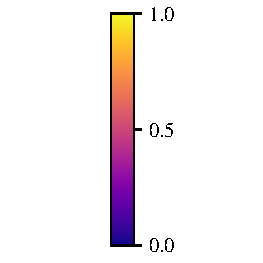
\includegraphics[width=0.3\textwidth]{papers/cahnhilliard/presentation/images/colorbar.book.pdf}}
\caption[Simulation der Cahn-Hilliard-Gleichung]{%
Simulation der Cahn-Hilliard-Gleichung über einen langen Zeitraum.}
\label{cahnhilliard:fig:chsim}
\end{figure}

\subsection{Ursache für die Entmischung}

\begin{figure}
\centering
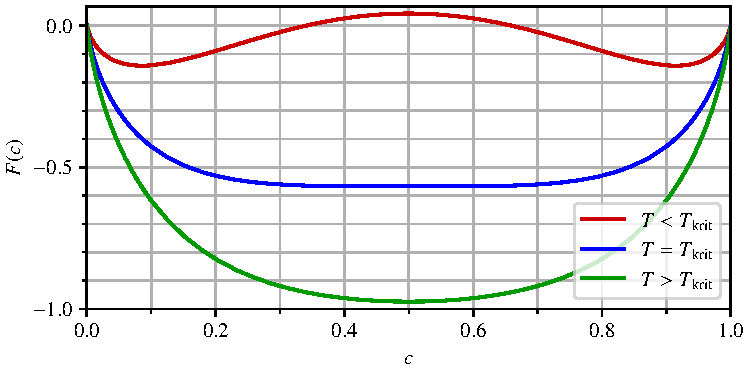
\includegraphics[scale=0.8]{papers/cahnhilliard/presentation/images/energy.book.pdf}
\caption{Temperaturabhängigkeit von $F(c)$}
\label{cahnhilliard:fig:fc}
\end{figure}

\begin{align*}
F(c)
&=
\Omega c (1 - c) + R T \left[ (1-c) \log(1-c) + c \log(c) \right]
\end{align*}

\begin{align*}
T_\text{krit}
&=
\frac{\Omega}{2 R}
\end{align*}
%
% \subsection{Gegenmassnahmen}
% \subsubsection{Rühren der Mischung}
% Verwenden wir nun die Integralform der Kontinuitätsgleichung.
% Anwenden Reynolds Transporttheorem (wichtiges Resultat der Fluiddynamik)
% Zeitableitung bedeutet hier zeitliche Ableitung des Materials.
% % TODO: Zitat / Quelle
% \begin{align*}
% \pderiv{}{t} \int_\Omega c \di{x}
% &=
% - \int_{\partial\Omega} \flux \cdot n \di{s}
% \\
% \int_\Omega \pderiv{c}{t} + \nabla \cdot (c v) \di{x}
% &=
% - \int_{\partial\Omega} \flux \cdot n \di{s}
% \end{align*}
% Nach anwenden des Divergenztheorems und da Geschwindigkeit divergenzfrei erhalten wir
% \begin{align*}
% \pderiv{c}{t} + v \cdot \nabla c
% &=
% \nabla \cdot (M \nabla \mu)
% \\
% \mu
% &=
% \deriv{F}{c} -  \epsilon^2 \Delta c
% \\
% \nabla \cdot v
% &=
% 0
% \end{align*}
% Zudem beschreiben wir den Einfluss des Rührprozesses über die periodischen Randbedinungen
% \begin{alignat*}{2}
% v_x(x, y, t)
% &=
% \alpha \sin(y + \phi_n)
% ,\quad&
% & n \tau \leq t < (n+1) \tau
% \\
% v_y(x, y, t)
% &=
% \alpha \sin(x + \psi_n)
% ,&
% & n \tau \leq t < (n+1) \tau
% \end{alignat*}
% \end{align*}
%
% TODO: Add plots of stirring process
